\appendix
\section{Technical details}
The results of this analysis have been obtained with the datasets listed in Table \ref{tab:datasets}.

\begin{table}[htbp]
\footnotesize

   \centering
   \begin{tabular}{llrrrrr}
     \toprule
     SAM definition & \phantom{a} & Events & \phantom{a} & POT & \phantom{a} & Scaling \\
     \midrule

     \verb|prodgenie_bnb_nu_cosmic_uboone_mcc8.7_reco2| & & 2156000 & & \num{2.10e21} & & 0.0206\\

     \verb|prodgenie_bnb_intrinsic_nue_cosmic_uboone_mcc8.7_reco2| & & 400000 & & \num{4.73e22} & & 0.00092\\
     
      \verb|prod_reco_optfilter_bnb_v12_unblind_mcc8_gooodruns_s| & & 171603 & & \num{4.36e19} & & 1\\
      
      \verb|prod_reco_optfilter_extbnb_v12_mcc8_gooodruns_s| & & 942165 & & \num{3.25e20} & & 0.134\\
     \bottomrule
   \end{tabular}
   \caption{SAM definitions for the data and Monte Carlo samples used in this analysis.}\label{tab:datasets}
\end{table}

The number of POT for each dataset has been measured with the script in \path{/uboone/app/users/zarko/getDataInfo.py}. The complete procedure is described in \cite{normalization}.

\section{Event displays}
In this section we show several event displays in the collection plane of simulated background and data events for each category.
\subsection*{Beam intrinsic $\nu_{\mu}$}
\begin{figure}[htbp]
\centering
  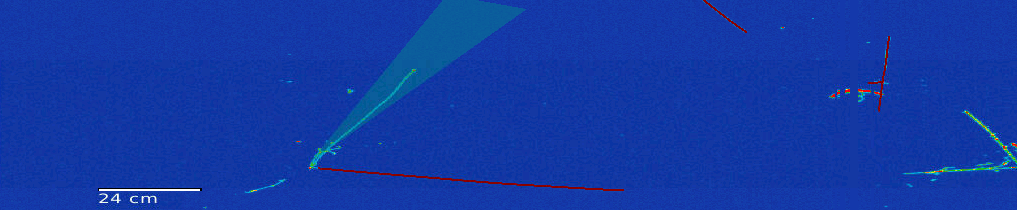
\includegraphics[width=0.75\linewidth]{evds/1_8845_442230_numu_kResCCNuProtonPiPlus.png}
  \caption{Beam intrinsic $\nu_{\mu}$ \texttt{kResCCNuProtonPiPlus}.}
\end{figure}

\begin{figure}[htbp]
\centering
  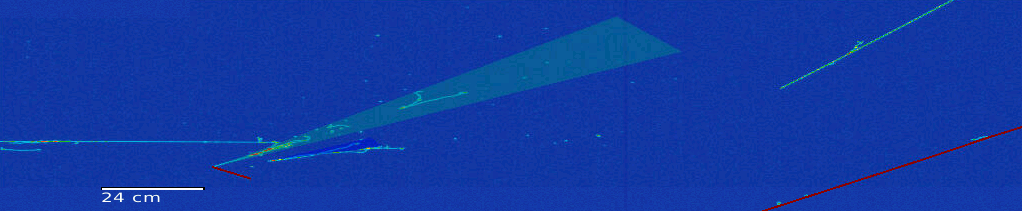
\includegraphics[width=0.75\linewidth]{evds/1_5848_292397_numu_kResCCNuNeutronPi0.png}
  \caption{Beam intrinsic $\nu_{\mu}$ \texttt{kResCCNuNeutronPi0}.}
\end{figure}

\subsection*{Beam intrinsic NC}

\begin{figure}[H]
\centering
  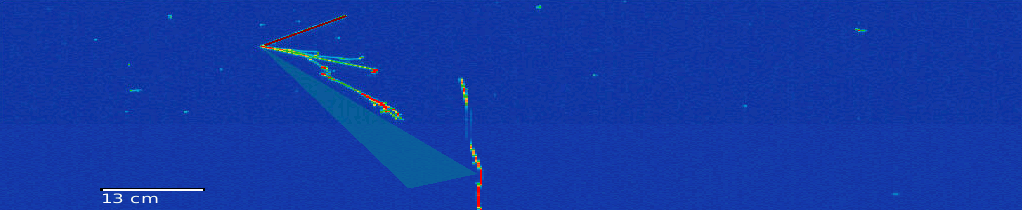
\includegraphics[width=0.75\linewidth]{evds/1_8996_449795_NC_kResNCNuNeutronPi0.png}
  \caption{Beam intrinsic NC \texttt{kResNCNuNeutronPi0}.}
\end{figure}

\begin{figure}[H]
\centering
  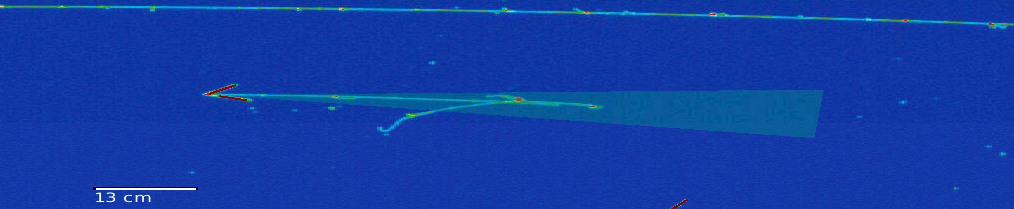
\includegraphics[width=0.75\linewidth]{evds/1_8275_413724_nc_kNCDIS.png}
  \caption{Beam intrinsic NC \texttt{kNCDIS}.}
\end{figure}

\subsection*{Cosmic contaminated}
\begin{figure}[H]
\centering
  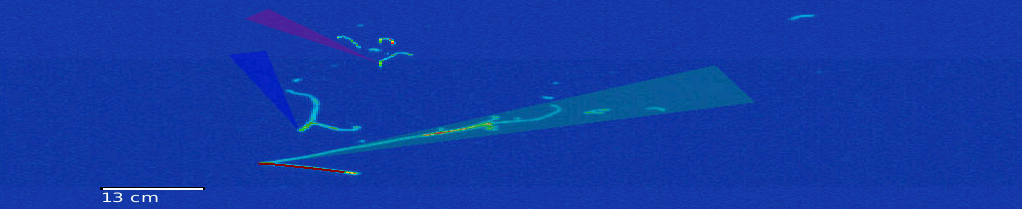
\includegraphics[width=0.75\linewidth]{evds/1_3458_172877_mixed_kResCCNuNeutronPi0.png}
  \caption{Cosmic contaminated.}
\end{figure}

\subsection*{Dirt}
\begin{figure}[H]
\centering
  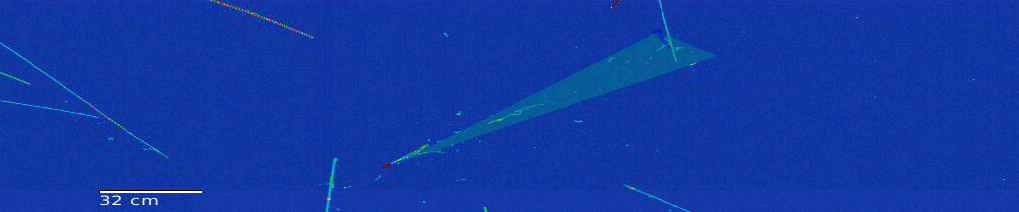
\includegraphics[width=0.75\linewidth]{evds/1_5516_275775_dirt_kResCCNuNeutronPi0.png}
  \caption{Dirt.}
\end{figure}

\subsection*{Cosmic in-time}
\begin{figure}[H]
\centering
  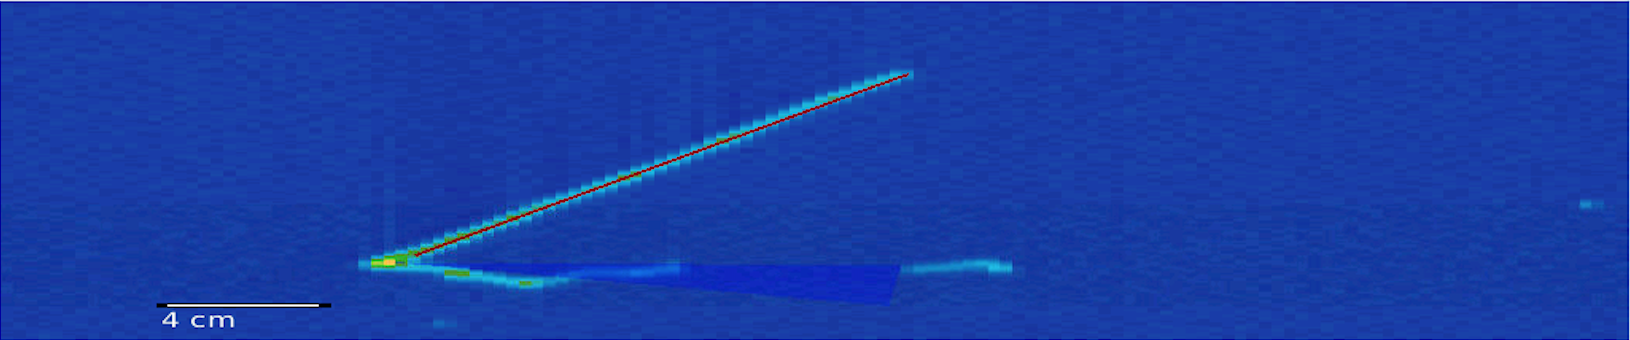
\includegraphics[width=0.75\linewidth]{evds/r5195_sr44_e2221.png}
  \caption{Cosmic in-time.}
\end{figure}

\subsection*{Cosmic}
\begin{figure}[H]
\centering
  
\includegraphics[width=0.75\linewidth]{evds/R5273_SR29_E1486.png}
  \caption{Cosmic ray.}
\end{figure}

\todo{Add event displays of background events}

